\section{Algorithmes cellulaires neuraux}

\par Les algorithmes cellulaires neuraux sont des automates cellulaires qui fonctionnent sur une grille bi dimensionnel de cellules contenant une valeur situé entre 0 et 1, et qui à l'aide d'une règle qui prend en compte les cases voisines d'une cellule via un voisinage de Moore, crée une grille où la règle a été appliqué à toutes les cellules de la grille de base. Le plus célèbre d'entre eux est bien sur le jeu de la vie, crée par John Conway, mais il est possible d'en faire une infinité d'algorithmes différents, dont les plus intéressant sont sur \href{https://neuralpatterns.io/}{ce site} (et c'est aussi la liste d'algorithmes que nous avons implémenté). 

\subsection{Fonctionnement}

\par Pour faire fonctionner un algorithme cellulaire neural, il faut avoir une règle, et une valeur qui est attribué a chaque cellule, qui sera déterminante pour appliquer la règle.

\par La règle est une fonction qui va prendre en entrée une valeur qui dépend de la \textbf{cellule principale} dont on veut changer la valeur mais aussi de son \textbf{voisinage} (les 8 cellules adjacentes orthogonalement ou diagonalement), et renvoie une nouvelle valeur pour la cellule principale, qui doit être comprise entre 0 et 1. La règle est inhérente à l'algorithme que l'on réalise, et peut ressembler à :
\begin{lstlisting}[language=Java]
public float regle(float x){
    if (x == 3f || x == 11f || x == 12f) return 1f;
    return 0f; }
\end{lstlisting}

\par Dans cet exemple, si la valeur donné en argument est 3, 11 ou 12, alors la règle renvoie 1, sinon 0. il n'y a pas de valeur intermédiaire, donc c'est équivalent au binaire, mais il est préférable d'utiliser des float car la plupart des algorithmes cellulaires neuraux ont besoin de float.

\par Pour ce qui est de la valeur associée à la cellule principale, la façon dont la valeur est calculé est par convolution avec une matrice de coefficients de taille 3 par 3: chaque coefficient est associé à une des cellules parmi la principale et son voisinage selon leur positionnement : un coefficient pour la cellule en haut a gauche de la cellule principale, un autre pour celle en dessous etc...

\par On va alors faire la somme de chaque multiplication de la valeur de la cellule et de son coefficient associé. On peut par exemple avoir une matrice de coefficients telle que :
\begin{table}[htp]
    \centering
    \begin{tabular}{|c|c|c|}
    \hline
    1&1&1\\
    \hline
    1&9&1\\
    \hline
    1&1&1\\
    \hline
    \end{tabular}
    \caption{Exemple de matrice de coefficients}
    \label{tab:tabCoef}
\end{table}
 \par Dans cet exemple simple de coefficients, si la cellule principale vaut 0 et que 5 de ces voisines valent 1 (le reste valant 0), alors la convolution vaudra 5. si la cellule principale vaut 1, et que 2 de ses voisines valent 1 (le reste valant 0), alors la convolution vaudra 11. C'est donc cette valeur qui sera donné à la règle pour déterminer la prochaine valeur de la cellule principale.

 \begin{figure}[H]
        \center
        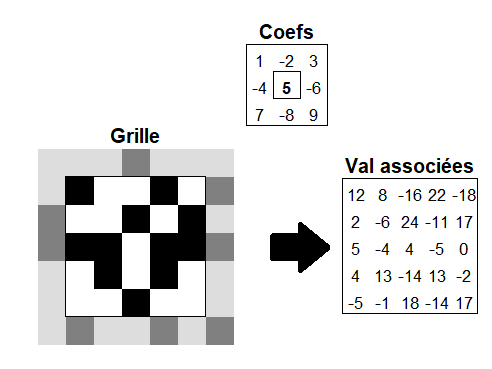
\includegraphics[scale=0.7]{images/imgAlgoNeural/IllustrationArbitraire.png}
        \caption{Illustration du fonctionnement avec des valeurs arbitraires}
\end{figure}
 
 \par \textbf{\textit{Totalement}} par coïncidence, la règle et les coefficients donnés en exemple sont ceux de Conway's Game Of Life : si une cellule est "morte" (vaut 0), alors la valeur x donné à la règle vaut entre 0 et 8, la cellule ne sera "vivante" (vaut 1) à la prochaine étape que si x vaut 3 donc si elle possède exactement 3 cellules voisines vivantes ; tandis que si elle est vivante, x vaut entre 9 et 17, elle ne sera vivante à la prochaine étape si x vaut 11 ou 12, donc si elle possède 2 ou 3 cellules voisines vivantes. A noter que si une cellule se trouve sur un des bords de la grille, les cellules situé sur le bord opposé de la grille peuvent être considéré comme parmi ses voisines ; ainsi toutes les cellules ont toujours 8 voisines.


\begin{figure}[H]
        \center
        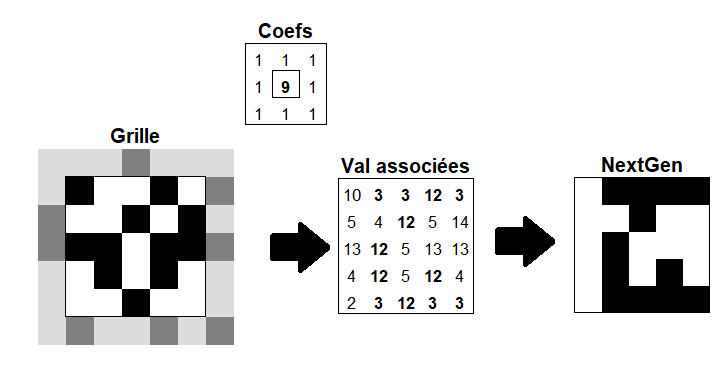
\includegraphics[scale=0.6]{images/imgAlgoNeural/IllustrationGOL.png}
        \caption{Illustration du fonctionnement avec le jeu de la vie}
\end{figure}
 
\par Ces règles peuvent être plus que de simples égalités, et vont souvent renvoyer une valeur entre 0 et 1, plutôt que seulement 0 et 1. Ainsi, avec une combinaison de règle et coefficients minutieuse, il est possible d'observer différents comportements d'algorithmes cellulaires neuraux.

\subsection{Implémentation}

\par \textit{Veuillez noter que, pour une partie des classes utilisées dans les algorithmes cellulaires neuraux et des voisinages de margolus, le nom de celles ci commence par "GOL", ce qui signifie "Game Of Life", et que c'est parfois un abus de langage car le projet porte sur le jeu de la vie, mais ce n'est pas pour autant que toutes les classes sont en rapport au jeu de la vie en tant que tel.}

\par Pour l'implémentation des algorithmes neuraux dans notre projet, on utilise une classe \textit{Grille}, qui est un tableau de taille par taille cellules, taille étant une constante donné à l'initialisation de la Grille, et chaque cellule étant un Float . \textit{Grille} implémente l'interface \textit{Univers}, qui est commun au principe de grilles et de quadtree. \textit{Grille} possède plusieurs méthodes, dont les principales sont \textit{getValAt}, \textit{setValAt}, et \textit{Afficher}. \textit{getValAt} retourne la valeur contenu dans la cellule dont on donne les coordonnées, \textit{setValAt} permet de remplacer les valeur dans une cellule dont on donne les coordonnées par une nouvelle valeur donnée, et \textit{Afficher} permet d'afficher la grille dans l'interface selon plusieurs arguments.

\par Cette \textit{Grille} est utilisé pour les algorithmes neuraux, via la classe \textit{GOLGrilleLifeLike}. Cette classe hérite de \textit{GOLGrille}, qui elle même hérite de la classe abstraite \textit{GOL}, qui sont 2 classes qui mettent les bases pour le fonctionnement des algorithmes neuraux, des voisinages de Margolus, mais aussi de Hashlife cependant uniquement pour la classe \textit{GOL}.

\par \textit{GOLGrilleLifeLike} a besoin de la taille, d'une règle, d'un mode, d'un randType, et optionnellement d'une couleur (qui n'est donc pas importante pour le fonctionnement de la classe) afin de faire fonctionner ses méthodes les plus importantes. Voici l'utilisation de ces variables, ainsi que les méthodes importantes :
\begin{itemize}
    \item La taille est la largeur et la hauteur de la grille, et cette dernière est créée dans le constructeur.
    \item La règle est utilisé pour créer une instance de \textit{DecodeGrilleLifeLike}, qui est une classe utilisé pour transformer la règle, qui est un String, en un tableau de coefficients, si la règle est conforme aux attentes pour une règle d'algorithmes neuraux : 9 nombres séparé par des "/", chaque nombre correspondant au coefficient pour l'une des positions de cellules pour la convolution.
    \item Le randType détermine, lorsqu'on tente de remplir la grille de valeur aléatoire via la méthode \textit{randomizeUnivers}, si la grille est rempli de 0 et de 1, ou si elle est rempli de valeurs flottantes entre 0 et 1, ou si la grille ne peut pas être rempli aléatoirement, en appelant respectivement les méthodes \textit{randomizeUniversBin}, \textit{randomizeUniversFloat}, ou aucun appel de méthodes. Le randType est utile car certains algorithmes fonctionnent sur des grilles où les valeurs ne peuvent avoir que 2 états, comme le jeu de la vie qui a des cellules qui ne peuvent être que "vivantes" ou "mortes", et d'autres qui sont adapté à avoir une situation initiale et ne pas être modifié via une grille aléatoire.
    \item Le mode est une valeur qui permet à la méthode \textit{tick} de savoir quel est l'algorithme neural qui dois être utilisé. La méthode \textit{tick} crée une nouvelle grille vide, et la rempli des valeurs de l'étape suivante de l'algorithme à l'aide du mode et du tableau de coefficient créé par l'instance de \textit{DecodeGrilleLifeLike}, et la renvoie.
    \item La couleur est un tableau de 3 valeurs entre 0 et 1, qui permettent d'accentuer une couleur lors de l'affichage de la grille (chaque valeur accentue respectivement le rouge, le vert, et le bleu). La plupart du temps, les valeurs sont de 0, ce qui permet un affichage en noir pour les cellules valant 1, blanc pour celles valant 0, et en teintes de gris pour les valeurs entre 0 et 1.
\end{itemize}

\par Ainsi, le fonctionnement des Algorithmes cellulaires neuraux est assuré par les méthodes décrites si dessus. Il est ensuite possible d'appeler depuis une classe qui coordonne toutes les autres classes une méthode \textit{update}, qui va changer la grille contenue dans l'instance de \textit{GOLGrilleLifeLike} en son étape suivante selon la méthode \textit{tick}, donc selon l'algorithme, et cette grille peut être affichée grâce à sa méthode \textit{Afficher}.

\begin{figure}[H]
        \center
        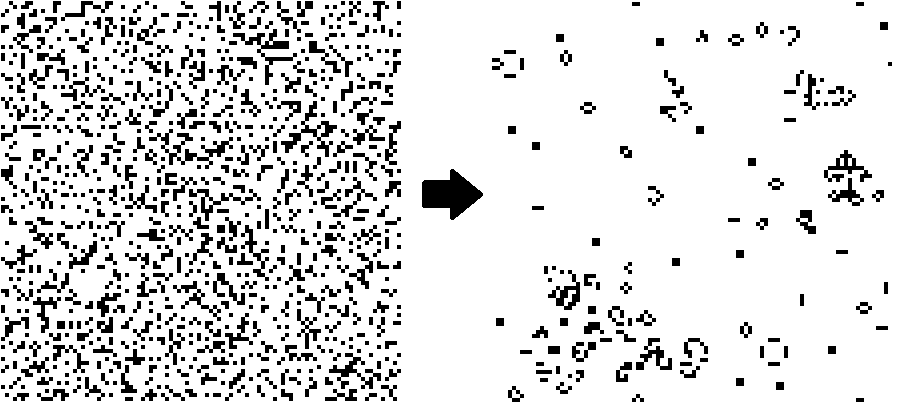
\includegraphics[scale=0.5]{images/imgAlgoNeural/GOLAvantApres.png}
        \caption{Jeu de la vie : début aléatoire $\rightarrow$ 1000 générations plus tard}
\end{figure}

\begin{figure}[H]
        \center
        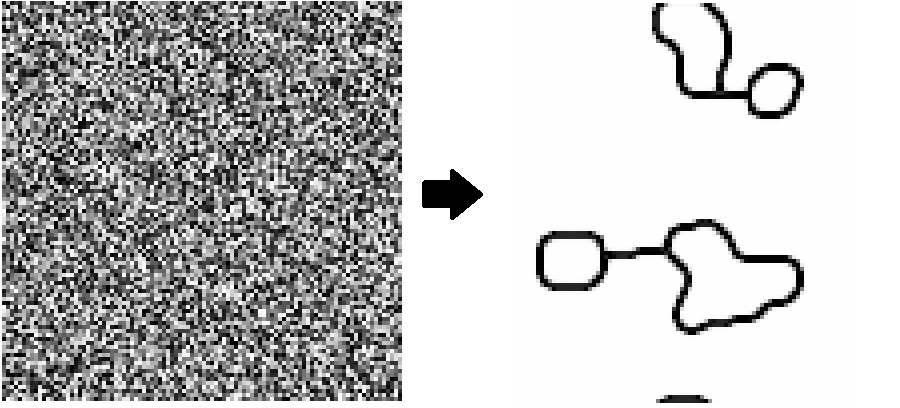
\includegraphics[scale=0.5]{images/imgAlgoNeural/PathwaysAvantApres.png}
        \caption{Algorithme Pathways : début aléatoire $\rightarrow$ 1000 générations plus tard}
\end{figure}